\cotefile{157-3}
\scanpage{130}
\mspage{79}

\uline{Remarque} La version duale \deleted{\unsure{du lieu|du lien}} (au sens de
Quillen) de l'axiome $\mathrm{W}(7\ \mathrm{bis})$ du carré cocartésien, i.e. l'axiome correspondant pour les
carrés cartésiens, n'est pas valable \deleted{\unsure{pour}} \unsure{$\mathcal W_\infty$}.
L'énoncé pertinent serait le suivant : soit

\diagram{\begin{tikzcd}[ampersand replacement=\&]
X \arrow[d,"f"'] \& X' \arrow[l,"q"'] \arrow[d,"f'"] \\
S \& S' \arrow[l,"p"']
\end{tikzcd}}

un carré cartésien, avec $f$ une \uline{$\mathcal W$-fibration}.
Alors $f\in\mathcal W\Longleftrightarrow f'\in\mathcal W$. Si \deleted{\unsure{Mais si on a seulement}
\unsure{soit} $f\in\mathcal W$} \unsure{:} \inserted{$\mathcal W$ satisfait} $\mathrm W(\unsure{4\,b|46})$\inserted{ (ce qui est le cas pour $\mathcal W_\infty$)}, alors $f\in\mathcal W$ implique
bien que ses fibres sont $\mathcal W$-asphériques, donc
que c'est une $\mathcal W$-équivalence universelle, i.e. $f'\in\mathcal W$
$\forall\,p:S'\unsure{-|\to}S$. Mais pour l'implication inverse
$f'\in\mathcal W\Rightarrow f\in\mathcal W$, il faut supposer \inserted{visiblement} que
\[
\pi_0(p):\pi_0(S')- \pi_0(S)
\]
est \uline{surjectif}. (P. ex. si $S'=\varnothing$, on a $X'=\varnothing$
donc $f'\in\mathcal W$, sans que ça implique $f\in\mathcal W$ !)

Le fait que dans le cas cocartésien de
$\mathrm W(7\ \mathrm{bis})$, $i_0\in\mathcal W\Rightarrow i\in\mathcal W$ doit être considéré
comme ``allant de soi'' -- autrement le carré
ne mérite pas, du point de vue $\mathcal W$-homotopique, le nom de ``cocartésien''. Par contre
l'implication inverse $\unsure{i|v}\in\mathcal W\unsure{\Longrightarrow|=}i_0\in\mathcal W$ m'apparaît comme un trait très particulier
du dérivateur $\mathrm{HOT}_{\mathcal W}$ (quand il le possède), et
notamment de $\mathrm{HOT}=\mathrm{HOT}_{\mathcal W_\infty}$. Le début

% archive sheet number: 130
\scanpage{131}
\mspage{80}

de la remarque \deleted{\unsure{doit}} signifie simplement que
le dérivateur dual $\mathrm{HOT}^{\circ}$ ne possède
pas cette même propriété. Je dois \unsure{envisager|renvoyer} à ce
sujet \deleted{\unsure{aux}} \deleted{\unsure{l'}}\inserted{deux} axiomes pour les dérivateurs correspondants à $\mathrm W(7\ \mathrm{bis})$, $\mathrm W(7)$, ce que je ferai
sans doute sous peu, de façon à donner
un sens plus précis au présent commentaire.

2.2. \uline{Application aux carrés cocartésiens déduits
d'une immersion ouverte ou fermée.}

Les axiomes $\mathrm W(7)$, $\mathrm W(7\ \mathrm{bis})$ (du \unsure{cube|crible}, \deleted{\unsure{carré}} et du
carré cocartésien) concernent des carrés cocartésiens
de nature très particulière. Nous allons
voir à présent comment en déduire des
énoncés \unsure{de|du} \unsure{=|même} type pour des carrés cocartésiens
beaucoup plus généraux, y compris pour des
carrés qui n'ont rien de cocartésien \inserted{(dans $\mathrm{Cat}$)} --
\deleted{\unsure{mais}} \inserted{et} que nous appellerons ``homotopiquement
cocartésiens'' (relativement à $\mathcal W$), ou simplement
\unsure{$\mathcal W$-cocartésiens}. (Il y aura également des carrés
$\mathcal W$-cartésiens un jour\ldots) Dans le cas où
$\mathcal W=\mathcal W_\infty$, je les appellerai \inserted{aussi} $\mathrm{Hot}$-cocartésiens.

Je commencerai par le cas particulier
d'un carré cocartésien associé à une \unsure{imm.|immersion}
ouverte, (diagramme \unsure{(5)|(*)|(6)} p.~74) :

\diagram{\(\text{(\unsure{*|**})}\qquad\begin{tikzcd}[ampersand replacement=\&]
U \arrow[r,hook,"i"] \arrow[d,"p"'] \& X \arrow[d,"q"] \& T \arrow[l,hook',dotted,"j"'] \arrow[d,dotted] \\
U' \arrow[r,hook,"i'"] \& X' \& T'\unsure{\simeq|=}T \arrow[l,hook',dotted,"j'"']
\end{tikzcd}\)}.

% archive sheet number: 131
\scanpage{132}
\mspage{81}

Le grand \unsure{traquenard} \inserted{ici} qu'il faut arriver à exorciser,
c'est qu'il peut arriver que $i\in\mathcal W$, sans qu'on
ait $i'\in\mathcal W$, et aussi $p\in\mathcal W$ sans qu'on ait $q\in\mathcal W$.
Je m'en étais convaincu en 1983 en écrivant
P.S. (\unsure{devant} les \unsure{sommations|miracles} du ``scratchwork''),
et n'ai pas envie de rechercher un \unsure{contrexemple|contre-exemple}
ici, s'il ne se présente de lui-même (ce
qu'il fera sans doute).

Je vais donner un cas important où ces
ennuis disparaissent :

\uline{Proposition} 6 : Considérons les adhérences $\overline U$
et $\overline U'$ de $U$ et $U'$ dans $X$, $X'$ respectivement,
et supposons que \deleted{$U\unsure{,|\to}\overline U$} les inclusions
\[
 U\xrightarrow{i_0}\overline U,\qquad U'\xrightarrow{i'_0}\overline U'
\]
soient \unsure{dans|des} $\mathcal W^{(*)}$. Alors
% slanted
\margin{cf th.~3 p.~47 \unsure{et} pour des conditions générales assurant que cette hypothèse \unsure{est|soit} satisfaite}
\[
\left\{\begin{aligned}
\text{\textcircled{a}}\, i\in\mathcal W&\Longleftrightarrow i'\in\mathcal W &&\text{si on a }\mathrm W(7\ \mathrm{bis})\\
\text{\textcircled{b}}\, p\in\mathcal W&\Longleftrightarrow q\in\mathcal W &&\text{si on a }\mathrm W(7).
\end{aligned}\right.
\]

Démonstration. \deleted{\unsure{La}}Considérons d'abord le cas \deleted{\unsure{a}}\textcircled{a} de
$\unsure{i_0|i}$, $i'$. Soit
\[
 k:\overline U\hookrightarrow X
\]
l'inclusion. Le triangle
\diagram{\begin{tikzcd}[ampersand replacement=\&]
 U \arrow[r,"i_0"] \arrow[rr,bend right=19,"i"'] \& \overline U \arrow[r,"k"] \& X
\end{tikzcd}}
, où $i_0\in\mathcal W$,
montre que $i\in\mathcal W\Longleftrightarrow k\in\mathcal W$. D'autre part $X$ est
la réunion des fermés $\overline U$, $T$, donc on a un
carré cocartésien dans $\mathrm{Cat}$
\diagram{\(\text{(*)}\qquad\begin{tikzcd}[ampersand replacement=\&]
 \overline U\cap T=\dot T \arrow[r,"k_0"] \arrow[d,"j_0"'] \& T \arrow[d,"j"]\\
 \overline U \arrow[r,"k"] \& X
\end{tikzcd}\)}
L'axiome $\mathrm W(7\ \mathrm{bis})$ (sous sa forme duale, (i.e. appliqué
au carré formé par les catégories opposées\ldots) implique

% archive sheet number: 132
\scanpage{133}
\mspage{82}

que
\[
 k\in\mathcal W\Longleftrightarrow k_0\in\mathcal W
\]
d'où
\[
 i\in\mathcal W\Longleftrightarrow(k_0:\dot T\to T)\in\mathcal W.
\]
De \unsure{=|même} \deleted{\unsure{pour}} on trouve\deleted{\unsure{r}}, en appliquant ceci à
$(X',U')$ au lieu de $(X,U)$
\[
 i'\in\mathcal W\Longleftrightarrow(k'_0:\dot T'\unsure{-|\to}T')\in\mathcal W.
\]
Or on a $T\xrightarrow{\sim}T'$ (\unsure{iso|isom}), et par la prop.~4
cet iso. transforme $\dot T$ en $\dot T'$. \deleted{D'où la conclusion}\inserted{Donc}
\[
 k_0\in\mathcal W\Longleftrightarrow k'_0\in\mathcal W\quad\text{(trivialement),}
\]
d'où a).

Prouvons b). Le carré comm. induit par $(*)$ p.~80
\diagram{\begin{tikzcd}[ampersand replacement=\&]
 U \arrow[d,"p"'] \& \overline U \arrow[l,"i_0"'] \arrow[d,"{\deleted{\unsure{q_{\overline U}|p_{\overline U}}}\overline p}"]\\
 U' \arrow[r,hook,"i'_0"] \& \overline U'
\end{tikzcd}}\noindent,
où $i_0,i'_0\in\mathcal W$ par hypothèse, montre que
\[
 p\in\mathcal W\Longleftrightarrow\overline p\deleted{\unsure{q_{\overline U}|p_{\overline U}}}\in\mathcal W,
\]
donc tout revient à prouver que
\[
 \overline p\in\mathcal W\overset{?}{\Longleftrightarrow}q\in\mathcal W.
\]
Mais $q$ induit un hom du carré $(*)$ déduit
de \deleted{$(X\unsure{,|q}\overline U,$} $(X,\overline U,T)$ (\unsure{avec|car} $X=\overline U\cup T$), dans le
carré similaire pour $X'$
\diagram{\begin{tikzcd}[ampersand replacement=\&]
 \overline U'\cap T'=\dot T' \arrow[r,"k'_0"] \arrow[d,"j'_0"'] \& T' \arrow[d,"j'"]\\
 \overline U' \arrow[r,"k'"] \& X'
\end{tikzcd}}\noindent,
les flèches verticales étant notées $q_{\dot T},q_T,\overline p\deleted{\unsure{q|U}},q$.

% archive sheet number: 133
\scanpage{134}
\mspage{83}

On sait que $q_{\dot T},q_T$ sont des iso, donc dans $\mathcal W$,
donc le ``lemme des cinq'' $\mathrm W(8)$ nous assure que
$\overline p\in\mathcal W\Longleftrightarrow q\unsure{,}\in\mathcal W$, qed.

\uline{Commentaire}. Cette proposition nous amène à
chercher des conditions sur un ouvert $U$ d'un
$X$, qui assurent que l'inclusion $i_0:U\to\overline U$
soit $\in\mathcal W$, et que \uline{cette propriété soit conservée
par tout cochangement de base} $U\unsure{-|\to}U'$. De
plus, nous recherchons des conditions qui soient
de nature locale sur $\overline U$, plus exactement sur
$\overline U\cap T=\dot U=\dot T$. Nous pouvons motiver ce
souci (a posteriori) en disant que nous
voudrions que la propriété $i_0\in\mathcal W$ soit conservée, non seulement par cochangement de base
\deleted{\unsure{que}}\inserted{quelconque} $U\to U'$, mais aussi, de plus, par
passage de $X$ à toute sous-catégorie pleine
$X_1$ contenant $U$, donnant donc naissance
à une situation
\[
 U\overset{\unsure{i_y|i_1}}{\subset} X_1,\qquad
 U\xrightarrow{(\unsure{d_y|i_y|i_1})_0}\overline U^{X_1}=\overline U\cap X_1
\]
\unsure{semblable|similaire} à la situation de départ. Plus
généralement encore, nous voudrions qu'elle
soit conservée en passant du \deleted{$(U,X)$}
triple $(X,U,T)$ à un triple ``induit'' $(X_1,U,T_1)$,
par \deleted{\unsure{la}} une \deleted{\unsure{fonction}}\inserted{flèche} quelconque $g:T_1\to T$ de
but $T$ dans $\mathrm{Cat}$, donnant naissance au
couple de flèches
\[
 U\xleftarrow{\mathrm{id}}U,\quad g:T_1\to T
\]
\unsure{cf pag|cf pp.} 60, 61). Le cas précédent est celui où

% archive sheet number: 134
\scanpage{135}
\mspage{84}

$T_1$ est une sous-catégorie pleine de $T$, $g$ la flèche
d'inclusion. Notons à ce sujet la proposition
suivante

\uline{Proposition} 7 Conditions équivalentes sur l'ouvert
$U$ d'un objet $X$ de $\mathrm{Cat}$ (moyennant $\mathrm W(7\ \mathrm{bis})$) :

a) l'inclusion $i_0:U\to\overline U$ est \deleted{dans $\mathcal W$}\inserted{$\mathcal W$-asphérique},
\deleted{\unsure{b)}} i.e. pour tout $t\in\dot U=\overline U\setminus U$, la catégorie
$U_{/t}$ est $\mathcal W$-asphérique.

b) L'inclusion $i_0:U\to\overline U$ est dans $\mathcal W$, et cette
condition reste satisfaite, quand on remplace
$(X,U)$ par $(X_1,U)$, où $(X_1,U)$ est déduit de
$(X,U)$ au moyen d'une flèche $T_1\to T$ $(=X\setminus U)$
dans $\mathrm{Cat}$, comme rappelé ci-dessus.

\deleted{b') \unsure{La condt} b), \unsure{est remplie|où on remplace} dans le cas où
$X_1$ est une sous-catégorie pleine de $X$ contenant $U$.}

b') Comme b), dans le cas où $T_1$ est la cat. ponctuelle $e$, et
\inserted{où de plus son image est dans $\dot U$.}

\deleted{b'') Comme b'), dans le cas où la sous-catégorie
pleine est de la forme $U\cup\{t\}$, avec $t\in\dot U$.}

\uline{Démonstration} : Il est évident que si dans b, b', b''
on remplace la condition ``$i_0\in\mathcal W$'' par \inserted{la condition plus forte} ``$i_0$ est
$\mathcal W$-asphérique'', les quatre conditions \deleted{\unsure{a) à}} b'') sont équivalentes. Il reste à prouver que
\unsure{la|les} condition\unsure{s} que les $U_{/t}$ soient $\mathcal W$-asphériques
($t\in\overline U$ -- mais c'est trivial pour $t\in U$, donc il
suffit de l'exprimer pour $t\in\overline U\setminus U=\dot U$)
est déjà impliquée par \deleted{\unsure{chacune des}}\inserted{la} plus faible, soit \unsure{b'} \deleted{\unsure{b''}},
et on devine qu'on a ceci :

\deleted{\uline{Corollaire 1} Soit $X_1\unsure{(t)|(b)}$ la sous-catégorie pleine}

% archive sheet number: 135
\scanpage{136}
\mspage{85}

\deleted{de $X$ dont l'ens. d'objets est $\mathrm{Ob}\,U\cup\{t\}$, où
$t$ \deleted{\unsure{$\in\dot U$|$\in\overline U$} \unsure{th.}} est un élément donné de $\dot U$. \deleted{Alors}
\unsure{(}Donc $U$ est un ouvert dans $X_1$, \deleted{\unsure{dense dans $X_1$},}
dont l'adh. dans $X_1$ est égale à $X_1$, et le
complémentaire est \deleted{la catégorie \unsure{ponc}} réduit à $t$.
Alors $U\xrightarrow{\unsure{i_1|i}}X_1$ est dans $\mathcal W$ sss $U_{/t}$ est
$\mathcal W$-asphérique. Même résultat pour la
catégorie $X'_1(t)$ définie par le foncteur
$e\to T$ d'image $t$ (comme dans b'').}

\deleted{Dém. Par construction, la catégorie $U_{/t}$
au sens du couple $(X,U)$ est isomorphe
à celle au sens du couple $(X_1(t),U)$, ou
du couple $(X'_1(t),U)$. Donc on est ramené
à ceci :}

\uline{Corollaire \deleted{\unsure{2}}} \inserted{(Moyennant $\mathrm W(7\ \mathrm{bis})$)}
Soit $X$ dans $\mathrm{Cat}$, $U$ un ouvert de $X$
tel que $X\setminus U=$\deleted{$\unsure{\overline{\{t\}}|\{t\}}$, et $X=\overline U$, \unsure{i.e.} $t\in\overline U$.}%
\inserted{soit la catégorie finale.}
Alors l'inclusion $U\overset{i}{\unsure{-|\to}}X$ est dans $\mathcal W$ sss
elle est $\mathcal W$-asphérique, i.e. sss $U_{/t}$ est $\mathcal W$-asphérique. (où $t$ est l'unique élément de $T$).

Nous démontrerons ultérieurement ce
corollaire\textsuperscript{*}.
% slanted
\margin{cf cor 4 de la prop.~15, page 149}
La prop.~7 ne nous servira pas
d'ici là -- elle n'aura qu'un rôle
purement \unsure{esthétique} à jouer, pour justifier
notre propos délibéré de chercher des
conditions sur $i:U\to X$ \deleted{\unsure{qui soient}}\inserted{\unsure{qui assurent|exprimant}}
que $U\to\overline U$ est dans $\mathcal W$ et le reste, \deleted{\unsure{par}}
quand on \deleted{fait bouger}\inserted{remplace} $(X,U)$ par d'autres
couples $(X_1,U_1\unsure{.})$ qui s'en déduisent par
certaines opérations \ldots) qui

% archive sheet number: 136
\scanpage{137}
\mspage{86}

soient de \uline{nature locale} sur $\overline U$ (en fait, en les
points de $\dot U$), et \deleted{plus précises qui} qui
\deleted{soient} en tout état de cause entraînent
la \inserted{$\mathcal W$-}\uline{asphéricité} de $U\to\overline U$.

J'avais espéré que cette condition d'asphéricité (suggérée par la notion ``d'immersion
de Dwyer'') serait stable par cochangement
de base quelconque $U\to U'$, ce qui aurait
assuré en même temps qu'après une telle
opération, la \inserted{l'immersion ouverte} $i':U'\unsure{-|\to}X'$ obtenue satisfait
encore à la condition que $i'_0:U'\to\overline U'$ est
dans $\mathcal W$. Nous verrons que cette attente n'est
pas fondée -- la condition de $\mathcal W$-asphéricité de $i$
n'est \uline{pas} stable par \unsure{cochangement} de base, et elle
ne suffit \uline{pas} \inserted{même} à assurer qu'après un \deleted{tel}
cochangement de base, $i'_0:U'\to\overline U'$ \unsure{``}soit dans $\mathcal W$.
Il faudra une notion plus forte, qui est
suggérée par le cas où $T$\inserted{$=\{t\}$} est la catégorie finale
\inserted{et contenue dans $\overline U$}
(\deleted{\unsure{au}} auquel nous avons essayé de nous ramener dans la \unsure{prop.}~7). Dans ce cas, on l'a dit \inserted{(corollaire précédent)},
la condition que $\unsure{i_0|i}:U\to\overline U$\inserted{$=X$} soit dans $\mathcal W$, équivaut
à la \inserted{$\mathcal W$-}asphéricité de $i$, i.e. à la \inserted{$\mathcal W$-}asphéricité de
$U_{/t}$, et de \unsure{=|même} pour $\unsure{i'|v'}:U'\to\overline U'=X'$ : elle
est dans $\mathcal W$ sss $U'_{/t'}$ est $\mathcal W$-asphérique, où

% archive sheet number: 137
\scanpage{138}
\mspage{87}

$t'$ est l'unique élément de $T'(\simeq T)\unsure{,}=X'\setminus U'$. Donc
il faut des conditions sur $U_{/t}$ \unsure{(?)} \deleted{\unsure{même}} qui
assurent que non seulement $U_{/t}$, mais aussi
toutes les catégories similaires $U'_{/t}$, soient
$\mathcal W$-asphériques. Dans le cas général \deleted{\unsure{de même}}\inserted{où}
$T$ est quelconque, c'est cette condition là que
nous allons imposer aux $U_{/t}$ $(t\in\mathrm{Ob}\,T)$, et il
s'avérera qu'\deleted{elles \unsure{sont}} cette fois-ci, \unsure{elles|elle} seront stables
par \inserted{tout} \unsure{cochangement|changement} de base $U\xrightarrow{p}U'$, i.e. que les
$U'_{/t'}$ $(t'\in\mathrm{Ob}\,T')$ satisferont alors à la \unsure{=|même} condition,
\inserted{C'est cette condition} que nous allons à présent reformuler.

2.3. \uline{Objets totalement $\mathcal W$-asphériques de} $\mathrm{Cat}$, \uline{et
morphismes totalement $\mathcal W$-asphériques.}

Reprenons la situation
\diagram{\begin{tikzcd}[ampersand replacement=\&]
 U \arrow[r,hook,"i"] \& X \& T \arrow[l,hook',"j"']
\end{tikzcd}}
, avec $T=\{t\}$, catégorie
finale \inserted{$t\in\overline U$, i.e. $X=\overline U$,} $e$,
et celle d'un $\mathrm{cochg}^{\mathrm t}$ de base $U\unsure{-|\to}U'$,
donnant naissance à un carré cocartésien dans $\mathrm{Cat}$ :
\diagram{\((\unsure{\alpha|1|*})\qquad\begin{tikzcd}[ampersand replacement=\&]
 U \arrow[r,hook,"i"] \arrow[d,"p"'] \& X \arrow[d,"q"'] \& T=\{t\} \arrow[l,dotted,hook',"j"'] \arrow[d,dotted,"\mathrm{iso}"] \\
 U' \arrow[r,hook,"i'"] \& X' \& T'=\{t'\} \arrow[l,dotted,hook',"j'"']
\end{tikzcd}\)}.
\deleted{Fixons nous \unsure{sur} le} \deleted{\unsure{Le|=} calcul de} La donnée de recollement $H$
entre $U$ et $T$, $H:\underbrace{U^{\circ}\times T}_{\simeq U^\circ}-\mathrm{Ens}$, \deleted{\unsure{peut}}
s'interprète comme un préfaisceau sur $U$,
\inserted{$H\in\mathrm{Ob}\,U^\wedge\ \unsure{{:}{:}|{:}}\ U^\circ\to\mathrm{Ens}$}

% archive sheet number: 138
\scanpage{139}
\mspage{88}

et on a
\[
 U_{/t}\simeq U_{/H},
\]
\unsure{et} $U_{/H}$ est interprété en termes du plongement
canonique
\[
 U\hookrightarrow U^\wedge\unsure{.|,}
\]
De \unsure{=|même}, le recollement entre $U'$ et $T'$ sera donné par un préfaisceau
\[
 H'\in\deleted{\unsure{U|U'}}\mathrm{Ob}\,U'^\wedge:\ U'^\circ\unsure{-|\to}\mathrm{Ens},
\]
et on aura
\[
 U'_{/t'}\simeq U_{/H'}.
\]
La relation entre $H'$ et $H$ a été explicitée
au \S~1 ; comme
\[
 H'=p_!H,\quad\text{où}\quad p_!:U^\wedge-U'^\wedge
\]
est l'adjoint à gauche de $p^*:U'^\wedge-U^\wedge$,
donné par
\[
 p^*F'=F'\circ p.
\]
On a
\[
 p_!(H)(u')\simeq\pi_0({}_{u'}\backslash U_{/H}).
\]

\uline{Définition} 1 : \textcircled{a} Soit $U$ un objet de $\mathrm{Cat}$,
$H$ \inserted{$\in\mathrm{Ob}\,U^\wedge$} un préfaisceau sur $U$. On dit que \deleted{\unsure{$F$|le}} $H$
est \uline{totalement} $\mathcal W$-\uline{asphérique} si pour toute
flèche $\unsure{p|f}:U\to U'$ de $\mathrm{Cat}$, $p_!(H)$ de $U'^\wedge$
est un objet $\mathcal W$-asphérique, i.e. $\unsure{W|U|U'}_{/p_!H}$ est
$\mathcal W$-asphérique. \textcircled{b} On dit qu'un objet $V$ de

% archive sheet number: 139
\scanpage{140}
\mspage{89}

$\mathrm{Cat}$ est \uline{totalement} $\mathcal W$-\uline{asphérique}, si le foncteur
final $\unsure{1|e}_V$ sur $V$ $(v\mapsto\{\varnothing\})$ est \deleted{\unsure{tota}} $\mathcal W$-asphérique,
i.e. si pour toute flèche $f:V\unsure{-|\to}V'$ dans $\mathrm{Cat}$,
le \deleted{foncteur} préfaisceau
\[
 \pi_0(f)\overset{\text{déf}}{=}\deleted{\unsure{p|f}}f_!(e_V)\overset{\text{déf}}{=}
 (v'\mapsto\pi_0({}_{v'}\backslash\unsure{X|V}))
\]
sur $V'$ est $\mathcal W$-asph, i.e. si la catégorie
\[
 \underline{\pi}_0(f)\quad\text{ou}\quad\underline{\pi}_0(V/V')
 \overset{\text{déf}}{=}V'_{/\deleted{\unsure{f}}\pi_0(f)}
\]
est $\mathcal W$-asphérique.

Notons que la \deleted{\unsure{constr}} définition des foncteurs
$p_!$ \inserted{(ou} $f_!$), \deleted{et leur} comme adjoints, et leur
``calcul'' en termes de $\pi_0$ de certaines catégories,
ne dépend pas du localiseur $\mathcal W$. Donnons
quelques précisions à ce sujet. On a un
morphisme d'adjonction dans $V^\wedge$
\[
 f^*f_!(F)\longleftarrow F,
\]
d'où
\[
 V_{/F}\longrightarrow V_{/f^*f_!(F)}\simeq V\times_{V'}(V'_{/f_!(F)}),\tag*{(*)}
\]
le dernier isomorphisme provenant du fait que
l'on a commutativité, à isom. can. près, dans
le diagramme de foncteurs
\diagram{\begin{tikzcd}[ampersand replacement=\&,column sep=huge,row sep=large]
 V'^\wedge \arrow[r,"{f^*=(F'\mapsto F'\circ f)}"] \arrow[d,"{F'\mapsto V'_{/F'}}"']
 \& V^\wedge \arrow[d,"{F\mapsto F_{/V}}"]\\
 \mathrm{Cat}_{/V'} \arrow[r,"{f^*_{\mathrm{Cat}}=(W'\mapsto W'\times_{V'}V)}"]
 \& \mathrm{Cat}_{/V}
\end{tikzcd}}\noindent,

% archive sheet number: 140
\scanpage{141}
\mspage{90}

en d'autres termes, l'opération $f^*$ sur les préfaisceaux s'interprète, en termes \unsure{géométrique|géométriques}, comme
l'opération $W'\mapsto W'\times_{V'}V$ de changement
de base par $V\unsure{-|\to}V'$, sur les catégories au
dessus de $V'$ qui sont fibrées à fibres discrètes (propriété qui se conserve par changement de base).

Ceci dit, la donnée d'une flèche
$(*)$ équivaut, par la propriété universelle
du changement de base, à celle d'une
flèche (canonique en l'\unsure{occurrence|occurence})
\[
 f_{/F}:V_{/F}\longrightarrow V'_{/f_!(F)}
\]
rendant commutatif le carré
\diagram{\((*)\qquad\begin{tikzcd}[ampersand replacement=\&,row sep=huge,column sep=huge]
 V_{/F} \arrow[r,"{\text{oubli de }F}","{\substack{\text{ou foncteur}\\\text{source}}}"'] \arrow[d,"{f_{/F}}"']
 \& V \arrow[d,"f"]\\
 V'_{/(F'\unsure{{:}{=}|{=}}f_!(F))} \arrow[r,"{\substack{\text{oubli de}\\ F'}}"]
 \& V'
\end{tikzcd}\)}.

Dans le cas qui nous intéresse surtout ici,
$F=e_V$, $V_{/F}\to V$ est un iso., et on
obtient une factorisation canonique de $f$ en

% archive sheet number: 141
\scanpage{142}
\mspage{91}

\diagram{\((**)\qquad\begin{tikzcd}[ampersand replacement=\&]
 \& V \arrow[dl,"{\widetilde f=f_{/e_V}}"'] \arrow[dd,"f","{\deleted{\unsure{V'|V}}}"{pos=.65,description}]\\
 \begin{gathered}\underline{\pi}_0(V/V')\\=V'_{/f_!(e_V)}\end{gathered} \arrow[dr,"\mathrm{can}"'] \& \\
 \& V'
\end{tikzcd}\)}.

Explicitons le $V'$-morphisme $\widetilde f$ sur les
fibres,
\[
 \widetilde f_{v'}:V_{v'}\longrightarrow
 \underline{\pi}_0(V/\unsure{v'|V'})_{v'}\overset{\text{déf}}{=}\pi_0({}_{v'}\backslash V),\tag*{(***)}
\]
où \inserted{dans} le \deleted{\unsure{deuxième}}\inserted{dernier} membre, on a identifié
l'ensemble $\pi_0({}_{v'}\backslash V)$ à la catégorie discrète
qu'il définit. Pour expliciter cette flèche
$(***)$, notons qu'on a une inclusion canonique
\[
 V_{v'}\longrightarrow{}_{v'}\backslash V
\]
et pour toute catégorie $W$, un morphisme
canonique (d'adjonction) $W\unsure{-|\to}\pi_0(W)$,
d'où un composé
\[
 V_{v'}-{}_{v'}\backslash V-\pi_0({}_{v'}\backslash V),
\]
qui n'est autre que $\widetilde f_{v'}$ dans $(***)$.

Il doit être facile de montrer que
la factorisation $(**)$ de $f$ est caractérisée,
à isom. \unsure{unique|uniques} près, \deleted{\unsure{par les}} en tant que

% archive sheet number: 142
\scanpage{143}
\mspage{92}

factorisation dans $\mathrm{Cat}_{/V'}$
\diagram{\begin{tikzcd}[ampersand replacement=\&,column sep=small]
 \& \widetilde V^{\deleted{\unsure{\prime|*}}} \arrow[dr,"\pi"] \&\\
 V^{\deleted{\unsure{\prime|*}}} \arrow[ur,"\widetilde f"] \arrow[rr,"f"'] \& \& V'
\end{tikzcd}}\noindent,
par les propriétés suivantes :

a) $\pi$ est \unsure{fibrant|fibrée} à fibres discrètes \inserted{i.e. un \deleted{\unsure{co}} iso. local}
(i.e. $\widetilde V^{\deleted{\unsure{\prime}}}$ est
isom. dans $\mathrm{Cat}_{/V'}$ à une catégorie $V_{/\unsure{F'|F_1}}$,
avec $F'$ dans $V'^\wedge$)

b) $\widetilde f_!(e_V)\simeq e_{\widetilde V}$, i.e. pour tout $\widetilde v\in\mathrm{Ob}\,\widetilde V$,
la catégorie $ {}_{\widetilde v}\backslash V$ est $0$-connexe : les
\deleted{dire que les} \unsure{colocalisées|colocalisations} de $V$ au dessus
de $\widetilde V$ sont $0$-connexes.

Notons ici, en passant, que pour \uline{tout} morphisme
$\pi:\unsure{\widetilde W'|W'}\unsure{-|\to}W$ dans $\mathrm{Cat}$ qui \deleted{soit} \unsure{fibre|fibré|fibrant} à fibres
discrètes, i.e. \inserted{tel que $W'$ soit} isom. \deleted{\unsure{dans $\mathrm{Cat}_{/W}$} \unsure{à un}}\inserted{dans $\mathrm{Cat}_{/W}$} à une
catégorie de la forme $W_{/F}$ $(F\in\mathrm{Ob}\,W^\wedge)$,
on a
\[
 \pi_!(e_{W'})=F,\ \text{i.e.}\quad W'\underset{\text{dans }\mathrm{Cat}_{/W}}{\simeq}W_{/\pi_!(e_{W'})}.\tag*{(*)}
\]
Il faut vérifier que le foncteur
\[
 w\mapsto\pi_0\bigl(\underbrace{{}_w\backslash(W_{/F})}_{\substack{\Vert\,\text{déf}\\ {}_{w\backslash}W_{/F}}}\bigr)
\]
est canoniquement iso. à $F$. Mais l'inclusion
\[
 \underset{\substack{\Vert\\ F(w)\\ \text{(cat. discrète)}}}{W'_w}\unsure{\longleftrightarrow|\longrightarrow|\hookrightarrow}{}_{w}\backslash W'
\]
\deleted{\unsure{définit bien|en fait bien|est un iso}}

% archive sheet number: 143
\scanpage{144}
\mspage{93}

définit bien comme tantôt
\[
 F(w)=W'_w\longrightarrow\pi_0(w\backslash W'),
\]
il faut prouver que c'est bijectif. Or, $W'$ étant
\deleted{lisse} $\mathcal W_\infty$-lisse sur $W$, on sait que l'inclusion
$W'_w\hookrightarrow{}_{w}\backslash W'$ est dans $\mathcal W_\infty$, a fortiori
induit un iso pour les $\pi_0$.

Ceci posé, si \inserted{on a} une factorisation de $f^{\unsure{\leftarrow|*}}\colon$\deleted{\unsure{$V\to$}} $V'$
en $f=\pi\widetilde f$ ayant les propriétés a) b) de
la page précédente, on voit déjà que l'on a
\[
 f_!(e_V)\simeq\pi_!\bigl(\underbrace{\widetilde f_{\unsure{!}}(e_V)}_{\substack{\Vert\\e_{\widetilde V}\ \text{par b)}}}\bigr)\simeq\pi_!(e_{\widetilde V}),
\]
ce qui déjà détermine $\widetilde V$ à isom. \unsure{canonique|canoniques}
près (grâce à a) comme
\[
 \widetilde V\simeq V'_{/f_!(e_V)}\overset{\text{déf}}{=}\underline{\pi}_0(V'/V),
\]
et il ne doit pas être bien dur de se
convaincre que $\widetilde f$ n'est autre que la \deleted{\unsure{flèche}}
flèche canonique de la page 91.

\uline{Proposition 8} Pour qu'un objet $H$ de $U^\wedge$

\figure{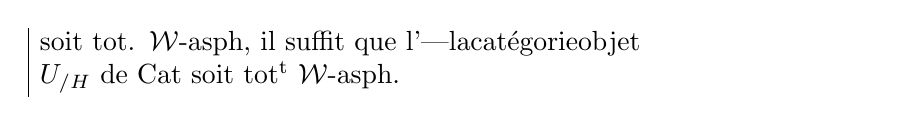
\begin{tikzpicture}
\node[anchor=north west,align=left,text width=.88\linewidth,inner xsep=4pt,inner ysep=1pt] (statement) at (0,0) {soit tot. $\mathcal W$-asph, il suffit que \unsure{l'|la}\deleted{catégorie}\inserted{objet}\\
$U_{/H}$ de $\mathrm{Cat}$ soit $\mathrm{tot}^{\mathrm t}$ $\mathcal W$-asph.};
\draw (statement.north west) -- (statement.south west);
\end{tikzpicture}}

% archive sheet number: 144
\scanpage{145}
\mspage{94}

Supposons en effet cette dernière condition satisfaite, et prouvons que $H$ est tot. $\mathcal W$-asphérique, i.e. que pour tout $p:U\unsure{-|\to}U'$, $U'/p_!(H)$ soit $\mathcal W$-asph.

\diagram{\begin{tikzcd}[ampersand replacement=\&]
V\overset{\text{déf}}{=}U_{/H}\arrow[r,"{\unsure{\alpha|p}}"]\arrow[dr,"f"'] \& U\arrow[d,"p"] \\
\& U'
\end{tikzcd}}

Soit $f$ le foncteur composé du diagramme ci-contre, on a $H\simeq\alpha_!(e_V)$ \deleted{\unsure{(par le|(par la}} (par $(*)$ p. 92), d'où
\[
p_!(H)\simeq p_!\alpha_!(e_V)\simeq(p\alpha)_!(e_V)\simeq f_!(e_V),
\]
qui est $\mathcal W$-asph. par hypothèse sur $V=U_{/H}$.

La réciproque de prop. 8 est-elle valable, i.e. si $H$ est totalement $\mathcal W$-asph., en est-il de \unsure{=|même} de $V=U_{/H}$ ? La difficulté provient du fait que \unsure{cela|cette} \deleted{\unsure{condition signifie|condition, signifie}} \inserted{signifie} que pour \uline{toute} flèche $f\inserted{{:}V\to V'}$ dans $\mathrm{Cat}$ de source $V$, on ait $f_!(e_V)$ $\mathcal W$-asphérique, alors que l'hypothèse \deleted{\unsure{ne pas|ne peut}} équivaut à le postuler seulement pour les flèches qui se factorisent par $U$. Notons que si on ne fait pas cette hypothèse sur $f$, mais \inserted{qu'on suppose} en lieu de cela que $f$ s'insère dans un carré commutatif

% archive sheet number: 145
